\chapter{Uživatelská příručka}
\label{sec:guide}

\section{První přihlášení}

\subsection{Změna hesla}

\begin{figure}[h!]
    \centering
    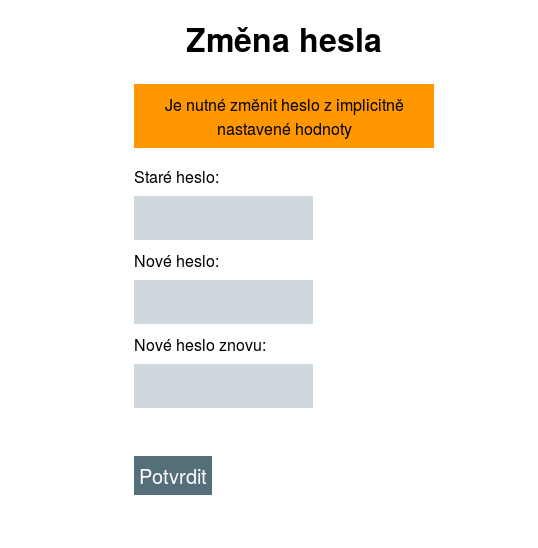
\includegraphics[width=0.7\textwidth]{images/pwd_change.png}
    \caption[Výzva ke změně hesla]{Výzva ke změně hesla}
    \label{fig:mvc}
\end{figure}

\section{Hlavní stránka}

\begin{figure}[h!]
    \centering
    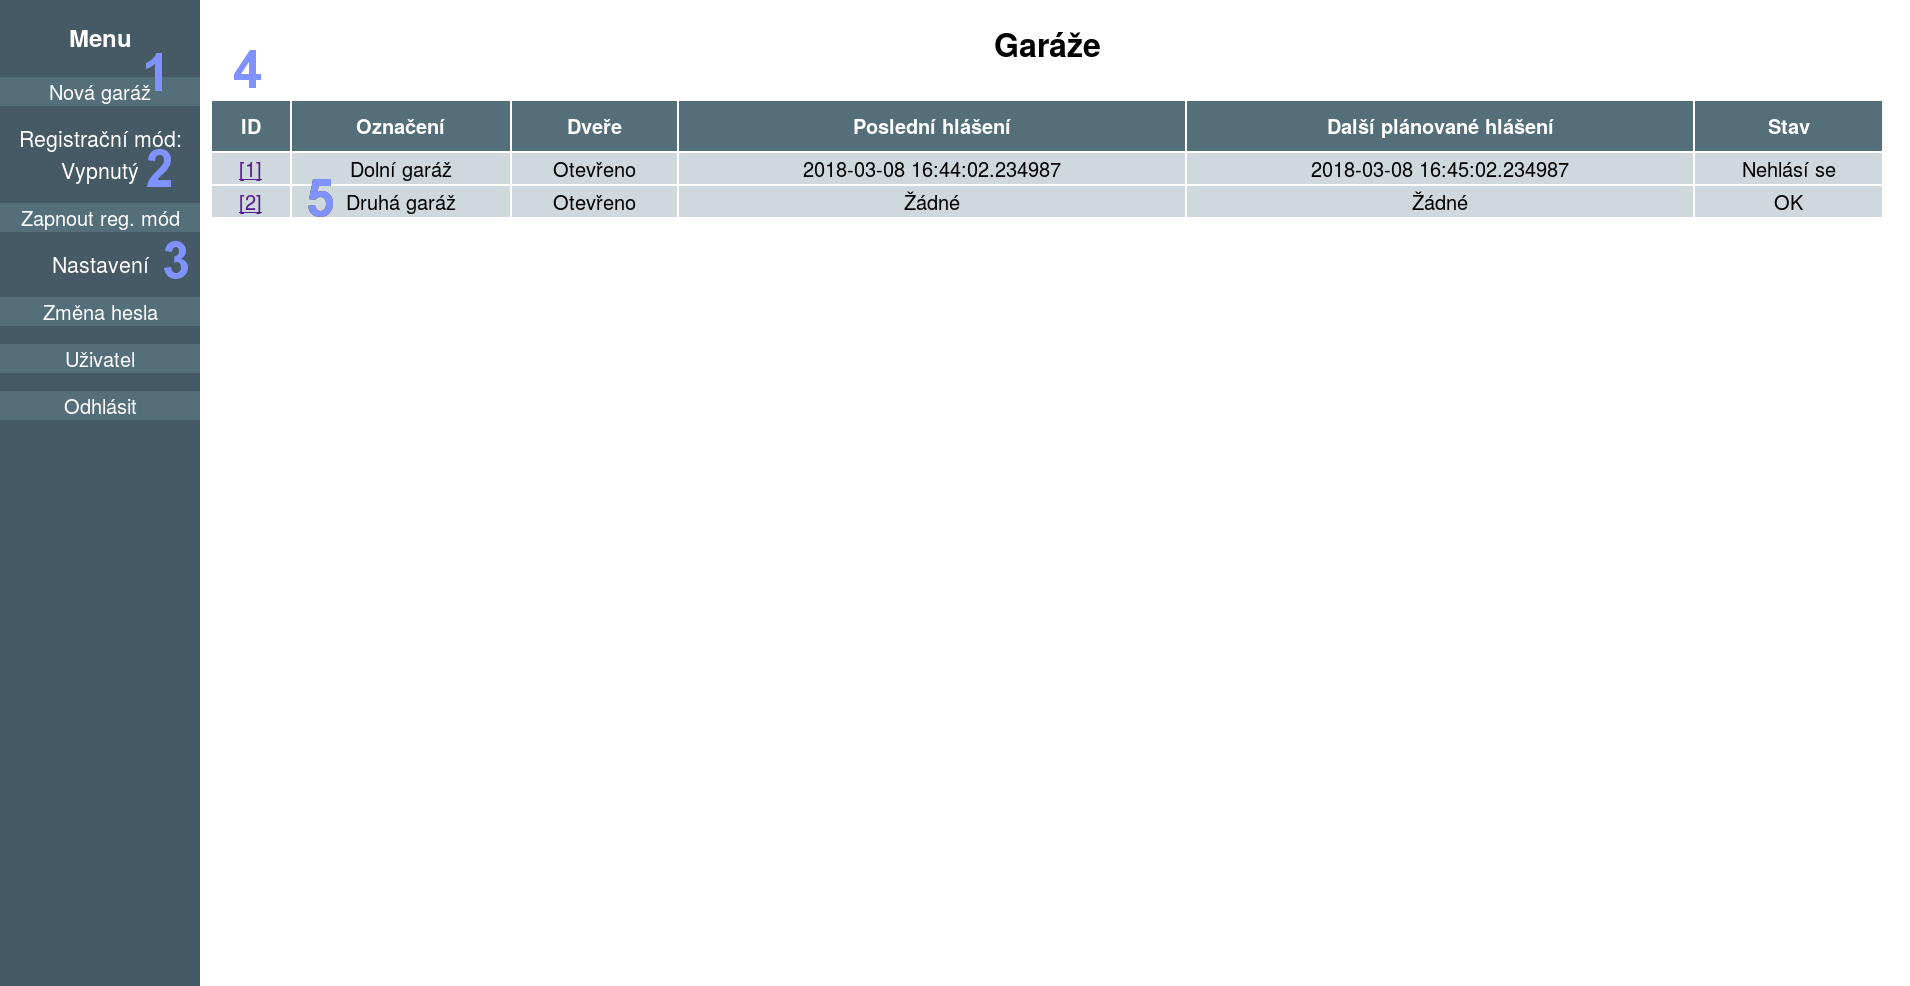
\includegraphics[width=\textwidth]{images/mainpage.png}
    \caption[Hlavní stránka aplikace]{Hlavní stránka aplikace}
    \label{fig:mainpage}
\end{figure}

Na obrázku \ref{fig:mainpage} je zobrazena hlavní stránka aplikace. Zde má uživatel k dispozici následující možnosti (viz čísla na obrázku):

\begin{enumerate}
    \item \textbf{Nová garáž} -- vytvoření nové garáže pomocí uživatelského rozhraní. Nová garáž je přidána do seznamu garáží na této stránce.
    \item \textbf{Registrační mód} -- indikátor stavu registračního módu. Regstrační mód povoluje podřízeným systémům vytvářet nové garáže registračním požadavkem. Při registraci pomocí tohoto módu je podřízenému systému automaticky zaslán API klíč, a není nutné ho ručně nahrávat.
    \item \textbf{Nastavení} -- uživatelské nastavení aplikace:
    \begin{itemize}
        \item \textbf{Změna hesla} -- možnost změny přístupového hesla do webového rozhraní.
        \item \textbf{Uživatel} -- viz sekci \ref{sec:guide_user_settings}.
        \item \textbf{Odhlásit} -- odhlášení z webového rozhraní.
    \end{itemize}
    \item Seznam sledovaných garáží (podřízených systémů):
    \begin{itemize}
        \item \textbf{ID} -- identifikátor garáže v systému, zároveň slouží jako odkaz na stránku garáže (viz sekci \ref{sec:guide_garage_page}).
        \item \textbf{Označení} -- Uživatelem zvolené označení garáže.
        \item \textbf{Dveře} -- Stav dveří garáže (otevřeno/zavřeno).
        \item \textbf{Poslední hlášení} -- Datum a čas posledního zaznamenaného hlášení.
        \item \textbf{Další plánované hlášení} -- Datum a čas dalšího plánovaného hlášení.
        \item \textbf{Stav} -- Stav garáže (OK, Nehlásí se, Detekce pohybu, Detekce kouře).
    \end{itemize}
    \item Záznam garáže.
\end{enumerate}

\section{Stránka garáže}
\label{sec:guide_garage_page}

\begin{figure}[h!]
    \centering
    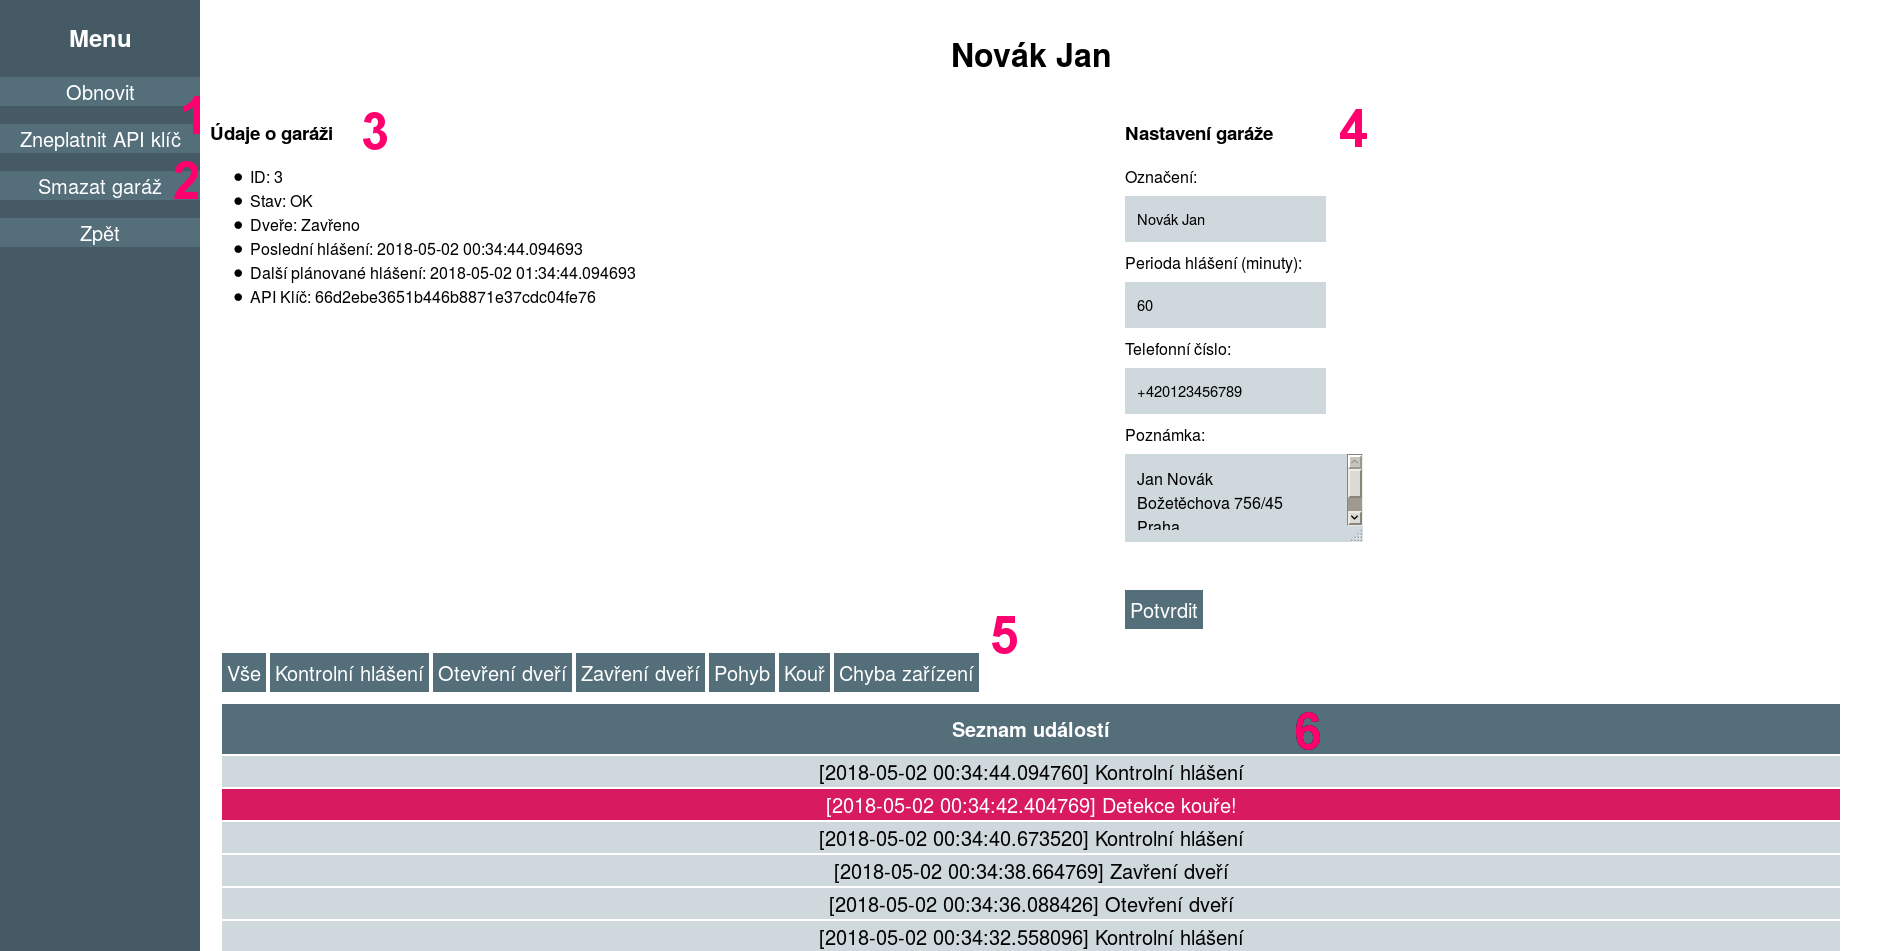
\includegraphics[width=\textwidth]{images/garage_page.png}
    \caption[Stránka garáže]{Stránka garáže}
    \label{fig:garage_page}
\end{figure}

Na obrázku \ref{fig:garage_page} je zobrazena stránka konkrétní garáže. Zde je možné provádět tyto operace:

\begin{enumerate}
    \item \textbf{Zneplatnit API klíč} -- vygeneruje nový API klíč garáže. Po jeho vygenerování již nebude podřízený systém v této garáži moci zasílat nové události. Pro obnovení přistupu je nutné nahrát na systém nový klíč, případně vytvořit novou garaž pomocí registračního módu.
    \item \textbf{Smazat garáž} -- smaže zobrazenou garáž, včetně zaznamenaných událostí.
    \item \textbf{Údaje o garáži}, včetně API klíče.
    \item \textbf{Nastavení garáže}:
    \begin{itemize}
        \item \textbf{Označení} -- uživatelem zvolené označení, které se zobrazí na hlavní stránce.
        \item \textbf{Perioda hlášení} -- perioda kontrolních hlášení podřízeného systému (v minutách).
        \item \textbf{Poznámka} -- volitelná poznánka ke garáži (max 256 znaků).
    \end{itemize}
    \item \textbf{Filtry událostí} -- možnost filtrovat zobrazené události podle typu.
    \item \textbf{Události} -- tabulka zaznamenaných událostí, včetně data a času.
\end{enumerate}


\section{Uživatelské nastavení}
\label{sec:guide_user_settings}